%!TEX root = ../dissertation.tex
\chapter{Perceptron e Sigmoid Neuron}

%\cite{Eigen1971, Knuth1968}.

\newthought{Introduzione alla Rete Neurale}

Cos'è una rete neurale? Per iniziare, spiegherò un tipo di neurone artificiale chiamato perceptron . Le perceptron furono sviluppate negli anni '50 e '60 dallo scienziato Frank Rosenblatt , ispirato ai precedenti lavori di Warren McCulloch e Walter Pitts . Oggi, è più comune usare altri modelli di neuroni artificiali - in questo libro, e in un lavoro molto moderno sulle reti neurali, il modello neuronale principale utilizzato è quello chiamato sigmoid neuron. Raggiungeremo a breve i sigmoid neurons. Ma per capire perché i sigmoid neurons sono definiti nel modo in cui sono, vale la pena prendersi il tempo per capire prima i perceptrons.
Quindi come funzionano i perceptron? Un perceptron accetta diversi input binari, x1, x2, … e produce una singola uscita binaria:

\begin{figure}
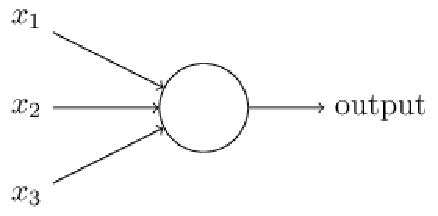
\includegraphics[width=%
0.5\textwidth]{figures/fig01}
\caption[Idea di un perceptron.]{Figura rappresentativa .
\label{fig:myInlineFigure}}
\end{figure}


Nell'esempio mostrato il perceptron ha tre ingressi, x1, x2, x3. In generale potrebbe avere più o meno input. Rosenblatt ha proposto una semplice regola per calcolare l'output. Ha introdotto pesi , w1, w2, … numeri reali che esprimono l'importanza dei rispettivi input per l'output. L'uscita del neurone, 0 o 1, è determinato dal fatto che la somma ponderata ΣjwjXj è minore o maggiore di qualche valore di soglia ( threshold value ). Proprio come i pesi, la soglia è un numero reale che è un parametro del neurone. Per metterlo in termini algebrici più precisi:

$$Output =
\bigg \{
\begin{array}{rl}
0 & \sum_j ( j \, w_j \, X_j ) \le threshold \\
1 & \sum_j ( j \, w_j \, X_j ) > threshold \\
\end{array}
$$

Questo è il modello matematico di base. Un modo in cui puoi pensare al perceptron è che è un dispositivo che prende le decisioni soppesando le prove e da cui, variando i pesi e la soglia, possiamo ottenere diversi modelli di decisione.

Per inciso, quando ho definito i perceptrons ho detto che un perceptron ha solo una singola uscita. Nella rete sopra i perceptron sembrano avere più uscite. In realtà, sono ancora a uscita singola. Le frecce di output multiple sono solo un modo utile per indicare che l'output di un perceptron viene utilizzato come input per molte altre percetron. È meno ingombrante del disegnare una singola linea di uscita che poi si divide.
Semplifichiamo il modo in cui descriviamo i peceptrons.
Il primo cambiamento è scrivere $\sum_j ( j \, w_j \, X_j )$ come prodotto, 
$ w \cdot x \equiv \sum_j ( j \, w_j \, X_j )$, dove w e x sono vettori i cui componenti sono rispettivamente i pesi e gli input. Il secondo cambiamento è spostare la soglia dall'altra parte della disuguaglianza e sostituirla con quella che è nota come bias del perceptron , $b \equiv -threshold$. Usando il bias invece della threshold, la formula del perceptron può essere riscritta:

$$Output =
\bigg \{
\begin{array}{rl}
0 & w\cdot X + b \le 0 \\
1 & w\cdot X + b > 0 \\
\end{array}
$$


Puoi pensare al bias come misura di quanto sia facile far percepire al perceptron un 1. O, per dirla in termini più biologici, la polarizzazione è una misura di quanto sia facile ottenere il perceptron a fuoco . Per un perceptron con una distorsione veramente grande, è estremamente facile per il perceptron emettere un 11. Ma se il bias è molto negativo, allora è difficile per il perceptrone emettere un 1. Ovviamente, introdurre il bias è solo un piccolo cambiamento nel modo in cui descriviamo i percetron, ma vedremo in seguito che questo porta a ulteriori semplificazioni notazionali. Per questo motivo, nel resto del libro non useremo la soglia, useremo sempre il bias.

Tuttavia, la situazione è migliore di quanto suggerisca questa visione. Si scopre che possiamo escogitare algoritmi di apprendimento in grado di sintonizzare automaticamente i pesi e le distorsioni di una rete di neuroni artificiali. Questa sintonizzazione avviene in risposta a stimoli esterni, senza l'intervento diretto di un programmatore.




\newthought{Sigmoid Neuron}

Per vedere come potrebbe funzionare l'apprendimento, supponiamo di fare un piccolo cambiamento in alcuni pesi (o bias) nella rete. Quello che vorremmo è che questo piccolo cambiamento di peso causi solo una piccola variazione corrispondente nell'output dalla rete. Come vedremo tra un momento, questa proprietà renderà possibile l'apprendimento. Schematicamente, ecco cosa vogliamo:

\begin{figure}
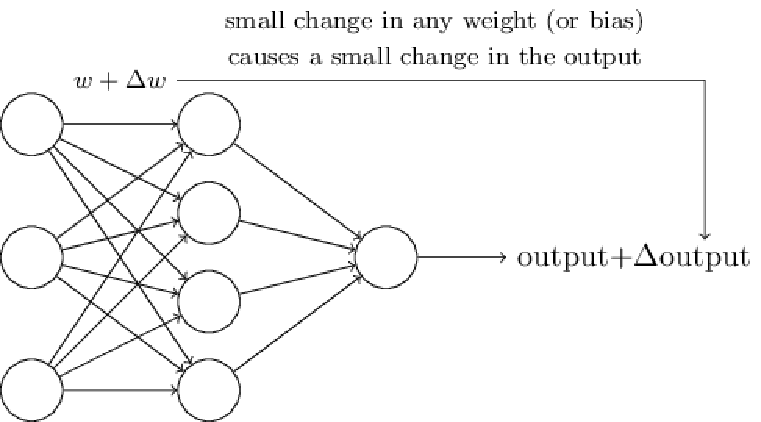
\includegraphics[width=%
0.8\textwidth]{figures/fig08}
\caption[Idea di un s.]{Figura rappresentativa .
\label{fig:myInlineFigure}}
\end{figure}

Se fosse vero che un piccolo cambiamento in un peso (o bias) causa solo un piccolo cambiamento nell'output, allora potremmo usare questo fatto per modificare i pesi e i bias per far sì che la nostra rete si comporti più nel modo che vogliamo. Poi lo ripetiamo, cambiando pesi e bias ripetutamente per produrre risultati migliori e migliori. La rete starebbe imparando.
Il problema è che questo non è ciò che accade quando la nostra rete contiene percetrons. In effetti, un piccolo cambiamento nei pesi o nei bias di ogni singolo perceptron nella rete può a volte far capovolgere completamente l'output di quel perceptron, diciamo da 0 a 1. Questo lancio potrebbe quindi far cambiare completamente il comportamento del resto della rete in un modo molto complicato. 
Ciò rende difficile vedere come modificare gradualmente i pesi e i bias in modo che la rete si avvicini al comportamento desiderato. Forse c'è un modo intelligente per aggirare questo problema. Ma non è immediatamente ovvio come possiamo ottenere una rete di percetrons da imparare.
Possiamo superare questo problema introducendo un nuovo tipo di neurone artificiale chiamato sigmoid neuron . I sigmoid neurons sono simili ai perceptrons, ma modificati in modo che piccoli cambiamenti nei loro pesi e bias causino solo un piccolo cambiamento nella loro produzione. Questo è il fatto cruciale che permetterà a una rete di sigmoid neurons di imparare. 
Descriveremo i sigmoid neurons nello stesso modo in cui abbiamo rappresentato i perceptrons:

Proprio come un perceptron, il sigmoid neuron ha input, x1, x2, … Ma invece di essere solo 0 o 1, questi input possono anche assumere qualsiasi valore compreso tra 0 e 1. Quindi, ad esempio, 0.638... è un input valido per un sigmoid neuron. Inoltre, proprio come un perceptron, il sigmoid neuron ha pesi per ogni input, w1, w2, … e un bias complessivo. Ma l'output non è 0 o 1. 
Invece, è σ ( w ⋅ x + b ), dove σ è chiamata la funzione sigmoide (sigmoid function) ed è definito da:\\

\begin{eqnarray} 
\sigma(z) \equiv \frac{1}{1 + e^{-z}}
\end{eqnarray}

Per dirla in modo un po' più esplicito, l'output di un sigmoid neuron con ingressi x1, x2, …, pesi w1, w2, … e bias b è : \\
\begin{eqnarray} 
\sigma(z) \equiv \frac{1}{1+\exp(-\sum_j w_j x_j-b)}
\end{eqnarray}


A prima vista, i sigmoid neurons appaiono molto diversi dai perceptrons. La forma algebrica della funzione sigmoide può sembrare opaca e proibitiva se non la conosci già. In effetti, ci sono molte somiglianze tra i perceptrons e i sigmoid neurons e la forma algebrica della funzione sigmoide risulta essere più un dettaglio tecnico che una vera barriera alla comprensione.
Per capire la somiglianza con il modello perceptron, supponiamo che 
$z \equiv  w \cdot x + b$ sia un grande numero positivo. Quindi $e^{-z} \approx 0$ e così $\sigma(z) \approx 1$.
In altre parole, quando $z= w \cdot x + b$ è grande e positivo, l'uscita dal sigmoid neuron è di circa 1, proprio come sarebbe stato per un perceptron. Supponiamo d'altra parte che $z = w \cdot x + b$ è molto negativo. Quindi $e^{-z} \to \infty$ e $\sigma(z) \approx 0$. Quindi, quando$ z= w \cdot x + b$ è molto negativo, anche il comportamento di un sigmoid neuron si avvicina molto a un perceptrons. È solo quando $z = w \cdot x + b$ è di dimensioni modeste che c'è molta deviazione dal modello perceptron.
Che dire della forma algebrica di $\sigma$? Come possiamo capirlo? In effetti, la forma esatta di σ non è così importante - ciò che conta davvero è la forma della funzione quando è tracciata. Ecco la forma:

\begin{figure}
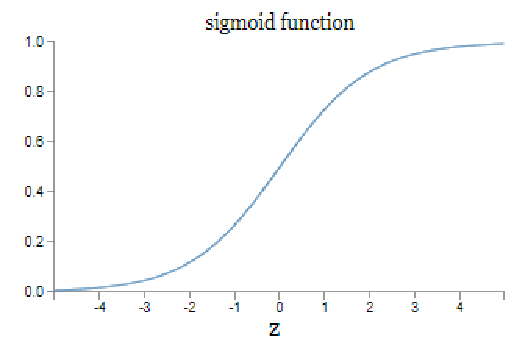
\includegraphics[width=%
0.8\textwidth]{figures/fig10}
\caption[Sigmoid function.]{Figura rappresentativa .
\label{fig:myInlineFigure}}
\end{figure}

Questa forma è una versione attenuata di una funzione di passaggio:

\begin{figure}
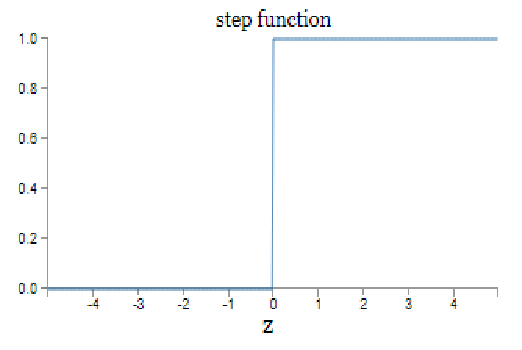
\includegraphics[width=%
0.8\textwidth]{figures/fig11}
\caption[Step function.]{Figura rappresentativa .
\label{fig:myInlineFigure}}
\end{figure}

Se σ era in effetti una funzione a gradino, allora il sigmoide sarebbe stato un perceptron, poiché l'output sarebbe 1 o 0 a seconda che w⋅x+b era positivo o negativo * . Usando il σ attuale la funzione che otteniamo, come già implicato sopra, è una percezione distorta. In effetti, è la scorrevolezza della funzione σ che è il fatto cruciale, non la sua forma dettagliata. La scorrevolezza di σ significa che piccoli cambiamenti Δwj nei pesi e Δb nel bias produrrà un piccolo cambiamento Δoutput nell'output dal neurone. In realtà, il calcolo ci dice che l' Δoutput è ben approssimato da

\begin{eqnarray} 
  \Delta \mbox{output} \approx \sum_j \frac{\partial \, \mbox{output}}{\partial w_j}
  \Delta w_j + \frac{\partial \, \mbox{output}}{\partial b} \Delta b
\end{eqnarray}


dove la somma è sopra tutti i pesi, $w_j$, e $\frac{\partial \, \mbox{output}}{\partial w_j}$ e $\frac{\partial \, \mbox{output}}{\partial b}$ denotano derivate parziali dell'output rispetto a $w_j$ e b, rispettivamente.
Mentre l'espressione sopra sembra complicata, con tutte le derivate parziali, in realtà sta dicendo qualcosa di molto semplice (e che è una buona notizia):

Δoutput è una funzione lineare dei cambiamenti $\Delta w_j$ e $\Delta b$ nei pesi e nei bias. Questa linearità semplifica la scelta di piccoli cambiamenti nei pesi e nei bias per ottenere qualsiasi piccola variazione desiderata nell'output. Quindi, mentre i sigmoid neurons hanno lo stesso comportamento qualitativo di perceptrons, rendono molto più facile capire come il cambiamento dei pesi e dei bias modificherà l'output.

Se è la forma di $\sigma$ che conta davvero, e non la sua forma esatta, allora perché usare la particolare forma usata per $\sigma$ in Equazione (2.1) ? In seguito calcolando le derivate parziali dell'Equazione (2.3), usando $\sigma$ semplificherà l'algebra. In ogni caso, $\sigma$ è comunemente usato nel lavoro sulle reti neurali, ed è la funzione di attivazione che useremo più spesso in questo libro.
Come dovremmo interpretare l'output di un sigmoid neuron? Ovviamente, una grande differenza tra perceptrons e sigmoid neurons è che i sigmoid neurons non producono solo 0 o 1. Possono avere come risultato qualsiasi numero reale tra 0 e 1, quindi valori come 0.173... e 0.689... sono uscite legittime. Questo può essere utile, per esempio, se vogliamo usare il valore di uscita per rappresentare l'intensità media dei pixel in un ingresso di immagine in una rete neurale. Ma a volte può essere una seccatura. Supponiamo di volere l'output dalla rete per indicare "l'immagine di input è un 9" o "l'immagine di input non è un 9". Ovviamente, sarebbe più semplice farlo se l'output fosse uno 0 o un 1, come in un perceptron. Ma in pratica possiamo stabilire una convenzione per affrontarla, ad esempio, decidendo di interpretare qualsiasi output di almeno 0,5 come indica un "9" e qualsiasi uscita inferiore a 0,5 come indicante "non un 9". Indicherò sempre esplicitamente quando usiamo tale convenzione, quindi non dovrebbe causare alcuna confusione.

% For an example of a full page figure, see Fig.~\ref{fig:myFullPageFigure}.

%% Requires fltpage2 package
%%
% \begin{FPfigure}
% 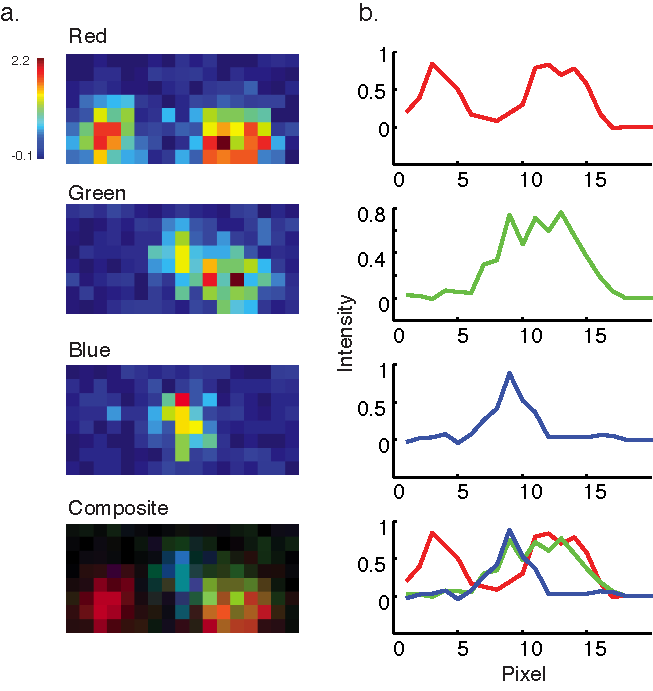
\includegraphics[width=\textwidth]{figures/fullpage}
%\caption[Short figure name.]{This is a full page figure using the FPfigure command. It takes up the whole page and the caption appears on the preceding page. Its useful for large figures. Harvard's rules about full page figures are tricky, but you don't have to worry about it because we took care of it for you. For example, the full figure is supposed to have a title in the same style as the caption but without the actual caption. The caption is supposed to appear alone on the preceding page with no other text. You do't have to worry about any of that. We have modified the fltpage package to make it work. This is a lengthy caption and it clearly would not fit on the same page as the figure. Note that you should only use the FPfigure command in instances where the figure really is too large. If the figure is small enough to fit by the caption than it does not produce the desired effect. Good luck with your thesis. I have to keep writing this to make the caption really long. LaTex is a lot of fun. You will enjoy working with it. Good luck on your post doctoral life! I am looking forward to mine. \label{fig:myFullPageFigure}}
 %\end{FPfigure}
 %\afterpage{\clearpage}

\newthought{Ottimizzazioni delle Sigmoid Neural Network}

Introduzione .................................

\newthought{Algoritmo di Backpropagation }

\begin{comment}
[RHW86] D. E. Rumelhart, G. E. Hinton, and R. J. Williams. Leaning Internal
Representaions by Ewvr Propagation in Rumelhart, D. E. and McClelland,
J. L., Pamllel Distributed Processing: Explorations in the Microstructure
of Cognition. MIT Press, Cambridge Massachusette, 1986.
\end{comment}

La regola delta generalizzata [RHW86], nota anche come algoritmo di propagazione posteriore (backpropagation), è spiegata qui brevemente per reti neurali con flusso in avanti ( feed-forward neural network).

%WIKI{https://it.wikipedia.org/wiki/Rete_neurale_feed-forward} prime 5 righe
In questa rete neurale le informazioni si muovono solo in una direzione, avanti, rispetto ai nodi d'ingresso, attraverso nodi nascosti (se esistenti) fino ai nodi d'uscita. Nella rete non ci sono cicli. Le reti feed-forward non hanno memoria di input avvenuti a tempi precedenti, per cui l'output è determinato solamente dall'attuale input.

%WIKI{https://it.wikipedia.org/wiki/Rete_neurale_artificiale}Storia
L'addestramento di une rete neurale di tipo backpropagation avviene in due diversi stadi: forward-pass e backward-pass. Nella prima fase i vettori in input sono applicati ai nodi in ingresso con una propagazione in avanti dei segnali attraverso ciascun livello della rete (forward-pass). Durante questa fase i valori dei pesi sinaptici sono tutti fissati. Nella seconda fase la risposta della rete viene confrontata con l'uscita desiderata ottenendo il segnale d'errore. L'errore calcolato è propagato nella direzione inversa rispetto a quella delle connessioni sinaptiche. I pesi sinaptici infine sono modificati in modo da minimizzare la differenza tra l'uscita attuale e l'uscita desiderata (backward-pass).

\begin{comment}
[RHW86] D. E. Rumelhart, G. E. Hinton, and R. J. Williams. Leaning Internal
Representaions by Ewvr Propagation in Rumelhart, D. E. and McClelland,
J. L., Pamllel Distributed Processing: Explorations in the Microstructure
of Cognition. MIT Press, Cambridge Massachusette, 1986.
\end{comment}

La spiegazione qui è destinata a fornire una descrizione del processo coinvolto nell'algoritmo di backpropagation usando, per semplicità, una rete neurale contente 3 livelli. Questi sono: livello di input, nascosto e di output.
Quindi, durante la fase di addestramento (training phase), i dati di addestramento (training data) vengono inseriti nel livello di input. I dati vengono propagati al livello nascosto e quindi al livello di output. Questo è chiamato il passaggio in avanti dell'algoritmo di backpropagation (forward-pass). 
In questo passaggio, ogni nodo nel livello nascosto ottiene input da tutti i nodi del livello di input, i quali vengono moltiplicati con pesi appropriati e quindi sommati. L'output del nodo nascosto è la trasformazione non lineare della somma risultante. 
Allo stesso modo ogni nodo nel livello di output riceve input da tutti i nodi del livello nascosto, che vengono moltiplicati con appropriati pesi e poi sommati. Nuovamente l'output di questo nodo è la trasformazione non lineare della somma risultante.
I valori di output del layer di output vengono confrontati con i valori di output di target (target output values).
I valori di output di target sono quelli che cerchiamo di insegnare alla nostra rete. L'errore tra i valori di output effettivi e i valori di output di target viene calcolato e propagato di nuovo verso il livello nascosto. 
Questo è chiamato backward-pass della rete. L'errore viene utilizzato migliorare la forza delle connessioni tra i nodi, ad es. le matrici di peso tra i livelli input-hidden e i livelli di output nascosti vengono aggiornate.

Durante la fase di test, non avviene alcun apprendimento, ad esempio, le matrici di peso non cambiano. Ogni vettore di prova viene inserito nel livello di input. L'avanzamento (feed-forward) dei dati di test è simile a quello dei dati nella fase di allenamento.

\newthought{Stochastic Gradient Descent}
Useremo la notazione x per denotare un input di formazione. Sarà conveniente considerare ogni input di allenamento x come vettore tridimensionale, l'output desiderato corrispondente di $y = y( x )$, dove y è anch'esso un vettore tridimensionale.
Quello che ci piacerebbe è un algoritmo che ci permetta di trovare pesi e bias in modo che l'output dalla rete si avvicini a y( x ) per tutti gli input di allenamento x. Per quantificare quanto bene stiamo raggiungendo questo obiettivo definiamo una funzione di costo:

\begin{eqnarray}  C(w,b) \equiv
  \frac{1}{2n} \sum_x \| y(x) - a\|^2.
\end{eqnarray}

Qui, w denota la raccolta di tutti i pesi nella rete, b tutti i bias, n è il numero totale di input di allenamento, a è il vettore di uscite dalla rete quando x è input, e la somma è su tutti gli input di training, x.
Ovviamente, l'output a dipende da x, w e b, ma per mantenere la notazione semplice non ho indicato esplicitamente questa dipendenza. La notazione || v || denota semplicemente la normale funzione di lunghezza per un vettore v. Chiameremo C la funzione di costo quadratico; a volte è anche noto come errore quadratico medio o solo MSE . 
Ispezionando la forma della funzione di costo quadratico, vediamo che C( w,b ) è non negativo, poiché ogni termine della somma è non negativo. Inoltre, il costo C( w,b ) diventa piccolo, cioè $C( w,b ) \approx 0$, precisamente quando y( x ) è approssimativamente uguale all'uscita, a, per tutti gli input di allenamento, x. Quindi il nostro algoritmo di allenamento ha fatto un buon lavoro se è in grado di trovare pesi e bias in modo che $C( w , b ) \approx 0$. Al contrario, non sta andando così bene quando C( w , b ) è grande, questo significherebbe che y( x ) non è vicino all'uscita a per un gran numero di ingressi. Quindi l'obiettivo del nostro algoritmo di allenamento sarà ridurre al minimo il costo C( w , b ) in funzione dei pesi e dei bias. In altre parole, vogliamo trovare una serie di pesi e bias che rendano il costo il più piccolo possibile. Lo faremo utilizzando un algoritmo noto come discesa del gradiente ( gradient descent ).

Abbiamo introdotto il costo quadratico perchè, utilizziamo una funzione di costo uniforme come il costo quadratico, risulta facile capire come apportare piccole modifiche nei pesi e nei bias in modo da ottenere un miglioramento nella funzione di costo.

Ricapitolando, il nostro obiettivo nell'addestrare una rete neurale è trovare pesi e bias che minimizzino la funzione di costo quadratico C( w , b ). Questo è un problema ben posto, ma ha una struttura molto distraente come è attualmente rappresentato, l'interpretazione di w e b come pesi e bias, il $\sigma$ funzione in agguato in background, la scelta dell'architettura di rete, i dati di input e così via. Si scopre che possiamo comprendere una quantità enorme ignorando la maggior parte di quella struttura e concentrandoci solo sull'aspetto di minimizzazione. Quindi per ora dimenticheremo tutto sulla forma specifica della funzione di costo, la connessione alle reti neurali ed il resto. Invece, immaginiamo di avere semplicemente una funzione di molte variabili e vogliamo minimizzare quella funzione. Svilupperemo una tecnica chiamata discesa del gradiente che può essere utilizzata per risolvere tali problemi di minimizzazione. Quindi torneremo alla funzione specifica che vogliamo minimizzare per le reti neurali.
Per ridurre al minimo C( v ) aiuta a immaginare C in funzione di due sole variabili, che chiameremo v1e v2:

Quello che vorremmo è trovare dove C raggiunge il suo minimo globale. Ora, ovviamente, per la funzione riportata sopra, possiamo guardare il grafico e trovare il minimo. In questo senso, ho forse mostrato una funzione leggermente troppo semplice! Una funzione generale, C, può essere una funzione complicata di molte variabili, e di solito non sarà possibile solo guardare il grafico a occhio per trovare il minimo.
Per le reti neurali spesso vogliamo molte più variabili - le reti neurali più grandi hanno funzioni di costo che dipendono da miliardi di pesi e bias in un modo estremamente complicato quindi usare il calcolo analitico per minimizzare non funzionerà!
Fortunatamente, esiste una bella analogia che suggerisce un algoritmo che funziona piuttosto bene.  

( STORIA DELLA PALLA )


\begin{comment}
Back Propagation Algorithm
The generalized delta rule [RHW86], also known as back propagation algorithm is explained here briefly for feed forward Neural Network (NN). The explanation here is intended to give an outline of the process involved in back propagation algorithm.
The NN explained here contains three layers. These are input, hidden, and output layers. During the training phase, the training data is fed into to the input layer. The data is propagated to the hidden layer and then to the output layer. This is called the forward pass of the back propagation algorithm. In forward pass, each node in
hidden layer gets input from all the nodes from input layer, which are multiplied with appropriate weights and then summed. The output of the hidden node is the nonlinear transformation of the this resulting sum. Similarly each node in output layer
gets input from all the nodes from hidden layer, which are multiplied with appropriate
weights and then summed. The output of this node is the non-linear transformation
of the resulting sum.
The output values of the output layer are compared with the target output values. The target output values are those that we attempt to teach our network. The error between actual output values and target output values is calculated and propagated
back toward hidden layer. This is called the backward pass of the back propagation
algorithm. The error is used to update the connection strengths between nodes, i.e.
weight matrices between input-hidden layers and hidden-output layers are updated.
During the testing phase, no learning takes place i.e., weight matrices are not
changed. Each test vector is fed into the input layer. The feed forward of the testing
data is similar to the feed forward of the training data.
\end{comment}

